\documentclass{article}
\usepackage{listings}
\usepackage[utf8]{inputenc}
\usepackage{ amssymb }
\usepackage{amsfonts}
\usepackage{graphicx}
\usepackage{boxproof}

\title{Lógica Matemática. \\Tarea 2}
\author{Fabián Romero Jiménez}
\date{}
\begin{document}
\maketitle
\begin{enumerate}

\item[\bf{Problema 1}] Di si las afirmaciones (a)–(d) son ciertas dado el marco siguiente:\\
El conjunto de mundos posibles $W = {A,B,C,D}$ y la relación de accesibilidad
$R = {(A,B), (C,D), (A,D), (A,A), (B,B), (C,C), (D,D)}.$\\
Además, tenemos la interpretación v:\\
$v(A, p) = F$ $v(B, p) = V$ $v(C, p) = F$ $v(D, p) = F$\\
$v(A, q) = F$ $v(B, q) = F$ $v(C, q) = V$ $v(D, q) = V$\\
$v(A, r) = F$ $v(B, r) = V$ $v(C, r) = F$ $v(D, r) = V$\\

\begin{center}
  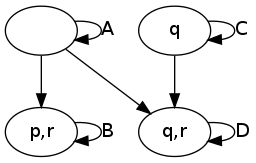
\includegraphics[scale=0.5]{graph1.png}\\
  Representación del modelo
\end{center}


\begin{itemize}
\item $A \models_v \Diamond (p \wedge q)$\\
Falso\\
Pues debería de existir un mundo accesible desde $A$ donde $p \wedge q$, ${A,B,D}$ son accecibles, pero $p$ solo se cumple en $B$ donde no se cumple $q$
\item $B \models_v \Box (q \leftrightarrow r)$\\
Falso\\
El único mundo accesible desde $B$ es el mismo, y ahí se cumple $r$ pero no $q$.
\item $\models_v \Box (p \rightarrow p)$\\
Es válido en general y por lo tanto válido en este modelo\\
pues ya sabemos que $p \rightarrow p$ es un teorema de lógica proposicional (para probarlo por deduccion natural, abrimos una caja con hipotesis $p$, por lo que $p$ es una conclusión válida dentro de la caja y por regla de introducción de la implicación se tiene $p \rightarrow p$) y por necesitación se tiene que $\Box (p \rightarrow p)$, por lo que es cierto para todo mundo en cualquier modelo.

\item $\models_v \Box (\neg q \wedge r)$\\
Falso\\
para que fuera válido en este modelo, en todo mundo accesible desde algún otro la fórmula habría de ser cierta por lo que $r$ debería de ser cierto, pero $r$ no es cierto en ${A,C}$ que son accesibles desde ellos mismos.
\end{itemize}

\item[\bf{Problema 2}] Sea $\mathcal{M} = \langle {a,b,c}), \mathcal{A} \rangle$ un marco. Dibuja algunas de las $\mathcal{A}$ posibles tales que $\mathcal{M}$ sea un modelo de:\\

\begin{enumerate}
\item $\Box\phi \implies \Diamond \phi$ ($S_1$  serial)\\
  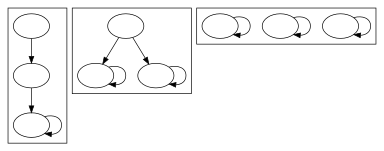
\includegraphics{e2a.png}\\

\item $\phi \implies \Box\Diamond \phi$ ($S_3$ simétrico)\\
  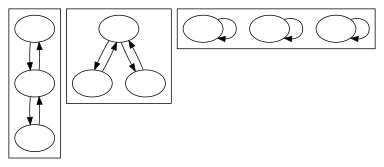
\includegraphics{e2b.png}\\

\newpage
\item $\Box\phi \implies \Box\Box\phi$ ($S_4$ transitivo)\\
  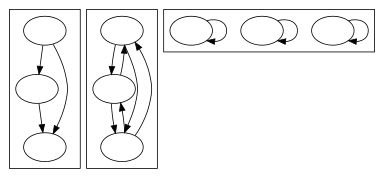
\includegraphics{e2c.png}\\

\item $\phi \implies \Box\phi$ (necesitación)\\
  Esto es cierto en cualquier modelo de Kripke, por lo que cualquier ejemplo dado en los otros incisos, sirve como ejemplo de esto.

\end{enumerate}

\item[\bf{Problema 3}]Demuestra que un marco cumple la propiedad\\

\begin{center}
  $ \forall u,v. u \rightarrow v \Rightarrow  v \rightarrow  u $\hspace{2 cm}($P_3$ simetría)
\end{center}
si y sólo si en ese marco es válida la fórmula
\begin{center}
  $S_3$  $\alpha \Rightarrow \Box\Diamond\alpha$\hspace{2 cm}$B(\alpha)$
\end{center}

\item[\bf{Demostración}]
($\Rightarrow$)\\
Sea $\mathcal(F)=(\mathcal{W},\mathcal{R})$ un modelo.\\
Suponga que $R$ es simetríca.
mostraremos que $\mathcal{M} \models \alpha \Rightarrow  \Box\Diamond \alpha$.\\
Es decir, que si $u \models \alpha$ entonces $\forall v. \mathcal{R}(u,v) (\exists z .\mathcal{R}(v,z).  z\models \alpha)$ 

sea $u\in \mathcal{W}$ un estado cualquiera en el cual $u \models \alpha$, para todo estado siguiente $v$, es decir $\forall v . \mathcal{R}(u,v)$ se tiene que $\mathcal{R}(v,u)$, pues $\mathcal{R}$ es simétrica, así, por lo que $\exists z. \mathcal{R}(y,x)$ donde $\alpha$ es válido, en este caso $z$ es $x$ $\blacksquare$ \\
($\Leftarrow$)\\
Supongamos que tenemos que $\alpha \Rightarrow \Box\Diamond\alpha$, por lo que en particular tenemos que $p \Rightarrow \Box\Diamond p$ para cualquier variable $p$, sea $\mathcal(L)$ una función de etiquetamiento tal que a cada estado le asigna una variable única, y sean $u,v . \mathcal{R}(u,v)$, supongamos que la variable en $u$ es $p$ como  $p \Rightarrow \Box\Diamond p$, pero el único estado donde $p$ es válido es en $u$, desde $v$ se tiene que $\Diamond p$, por lo que necesariamente es cierto que $\mathcal{R}(v,u)$ y por lo tanto la relación es simétrica $\blacksquare$


\item[\bf{Problema 4}] Da una estructura de Kripke de un sistema con dos agentes, cada uno de los cuales tiene como estado un vector de tres bits. Cada agente sabe que el estado del otro agente difiere del suyo en el valor de exactamente un bit, pero no sabe cuál.

\begin{center}
  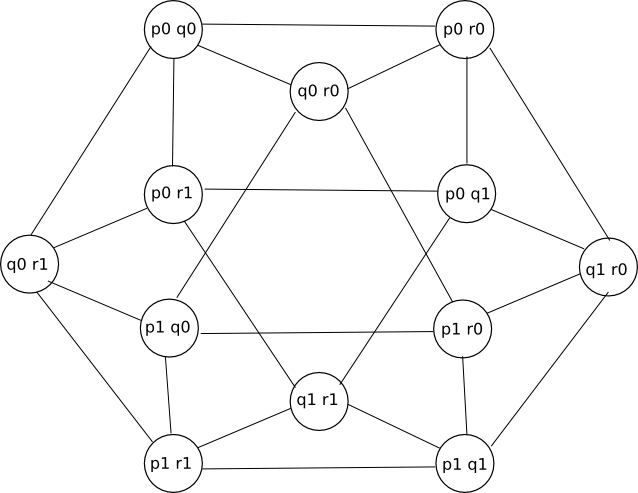
\includegraphics[scale=0.5]{e4_4.png}\\
\end{center}

El modelo aqui presentado tiene 12 estados, es decir 12 mundos posibles en cada uno de ellos, los agentes concuerdan en 2 bits, donde el orden del bit lo representamos con la letra p,q y r y el valor con el dígito 0 o 1, asi un estado representa dos bits de acuerdo.

La relación de accesibilidad es simétrica, por lo que no ponemos dirección en las aristas, y cada estado es accesible desde otros 4 estados que son aquellos donde esta presente el bit sobre el cual no hay acuerdo (en ambos valores 0 y 1) y uno de los 2 bits que si estan de acuerdo (con el valor fijo que tiene en el estado). 


\item[\bf{Problema 5}]  Considera el problema de los niños lodosos visto en clase. La variable $m_i$ denota que el niño $i$ está lodoso. Sea $\Gamma$ la conjunción de las siguientes
fórmulas:

$$C(m_1 \vee m_2 \vee .. \vee  m_n)$$\\
$$ \bigwedge\limits_{i\neq j}C(m_i \rightarrow K_jm_i) $$\\
$$ \bigwedge\limits_{i\neq j}C(\neg m_i \rightarrow K_j \neg m_i) $$\\
Sea $G$ cualquier conjunto de niños, y
$$  \alpha_G = \bigwedge\limits_{i\in G} m_i  \wedge \bigwedge\limits_{i \not \in G} \neg m_i $$

Es decir, $\alpha_G$ afirma que exactamente los niños en $G$ están lodosos.\\
Usando deducción natural, demuestra que:

$$  \Gamma,\alpha_{\{i\}} \models K_im_i$$\\

que corresponde con la situación en la que si exactamente un niño está
lodoso, ese niño lo sabe.

\item[\bf{Demostración}]

Primero probemos que:\\
 $\vdash_N  (\neg b) \wedge ( a \vee b )  \rightarrow a $\\

\begin{proofbox}
  \[
  \lbl{1}\:    (\neg b) \land (a \lor b)            \= \mbox{Hipótesis}\\
  \lbl{2}\:    \neg b                               \= \elim\land(\ref{1})  \\
  \lbl{3}\:    a \lor b                             \= \elim\land(\ref{1})  \\
  \[
  \lbl{4}\:    a                                    \= \mbox{Hipótesis}\\    
  \]
  \[
  \lbl{5}\:    b                                    \= \mbox{Hipótesis}\\    
  \lbl{6}\:    b \land  \neg b                      \= \intro\land(\ref{6},\ref{2}) \\
  \lbl{7}\:    a                                 \= \mbox{F(7)}\\    
  \]
  \lbl{8}\:    a                                 \= \elim\lor(4,7) \\
  \]
  \lbl{9}\:    (\neg b) \land (a \lor b) \to a   \= \intro\to  \\
\end{proofbox}\\

Ahora, si exactamente un niño esta lodoso tenemos que:\\
$$  \alpha_G = \bigwedge\limits_{i\in G} m_i  \wedge \bigwedge\limits_{i \not \in G} \neg m_i $$
si el niño lodoso es el $i$
$$  \alpha_G =  m_i  \wedge \bigwedge\limits_{i \not \in G} \neg m_i $$
y dado que:
$$ \bigwedge\limits_{i\neq j}C(m_i \rightarrow K_jm_i) $$\\

usando $a$ como la interpretacion de $m_i$, y b como $ \bigwedge\limits_{i\neq j}C(m_i \rightarrow K_jm_i) $\\
y dado que $\Gamma$ es la conjunción de las formulas tenemos:
 $(\neg b) \wedge ( a \vee b ) $\\
pero por nuestra prueba de deducción natural y aplicando modus ponens tenemos
$a$, cuya interpretacion $m_i$ es precisamente que el único niño lodoso, sabe que lo está.
\end{enumerate}
\end{document}
